% !Mode:: "TeX:UTF-8"
\documentclass[QA.tex]{subfiles}
\begin{filecontents*}{MWE_array_colortbl.tex}
%MWE_array_colortbl.tex
\documentclass[11pt,a4paper]{memoir}
%\usepackage{array}
%\usepackage{xcolor}
%%----colortbl 与 memoir 中的array环境冲突-------
%colortbl 要求array 及 color 包。
%\usepackage{colortbl}
%色彩表格\columncolor,\rowcolor,\cellcolor,\rowcolors
\begin{document}
	\[
	\begin{array}({cc})
	a & b\\ c & d
	\end{array}
	\]
	\[
	\begin{array}[c]({c})
	\begin{array}[c]|{cc}|
	x_1 & x_2\\
	x_3 & x_4
	\end{array}\\
	y\\
	z
	\end{array}
	\]
\end{document}
\end{filecontents*}
\begin{document}
%-=-=-=-=-=-=-=-=-=-=-=-=-=-=-=-=-=-=-=-=-=-=-=-=
%
%	CHAPTER
%
%-=-=-=-=-=-=-=-=-=-=-=-=-=-=-=-=-=-=-=-=-=-=-=-=

%%================================================================
\chapter{20180404}\label{ch180404}
%----------------------------------------------------------------------------------------

\begin{qst}\label{Q2018040401}
 如何在行内插入命令?就是直接显示\verb+\|%+ 等符号?\index{行内verb}
\end{qst}
\ans 可以使用\mintinline{tex}{\verb+\|%+}或者\mintinline{tex}{\mintinline{tex}{\|%}}。
		

\begin{qst}\label{Q2018040402}
 verb不能在frame环境里用啊?\index{beamer用verb}
\end{qst}
\ans beamer的frame后加个[fragile]就好了。

\begin{qst}\label{Q2018040403}
 请问一下\TeX{}Live是用命令行安装的么?
\end{qst}
\ans \TeX{}Live可以不用命令行安装,也可以用命令行安装。如果没记错的话,安装命令是install-tl-windows.bat -no-gui。

\begin{qst}\label{Q2018040404}
 运行以下mwe, 如果将\mintinline{tex}{%\usepackage{colortbl}}打开,则运行出错;
	如果将注释掉colortbl包,则运行正常。
 我想用colortbl包的色彩表格功能,同时也用到memoir文档类扩充的array数学环境。
 请问如何兼得呢。
 \inputminted[linenos]{tex}{MWE_array_colortbl.tex}
 \end{qst}
\ans 这两个宏包并不冲突,是用法不对。
 \begin{minted}{tex}
 \newcolumntype{C}{>{$}c<{$}}
 \[
   \left(
   \begin{tabular}{C>{\columncolor{gray}[0pt]}C}
     \rowcolor{green}[0pt]a & b\\ c & d
   \end{tabular}
   \right)
 \]
 \end{minted}
 \newcolumntype{C}{>{$}c<{$}}
  \[
   \left(
   \begin{tabular}{C>{\columncolor{gray}[0pt]}C}
     \rowcolor{green}[0pt]a & b\\ c & d
   \end{tabular}
   \right)
 \]
 \begin{minted}{tex}
  \[
    \left(
    \begin{tabular}{C>{\columncolor{gray}[0pt]}C}
      x_1 & x_2\\
      \rowcolor{yellow}[0pt]x_3 & x_4
    \end{tabular}
    \right)
 \]
 \end{minted}
  \[
   \left(
   \begin{tabular}{C>{\columncolor{gray}[0pt]}C}
     x_1 & x_2\\
     \rowcolor{yellow}[0pt]x_3 & x_4
   \end{tabular}
   \right)
 \]
 \begin{minted}{tex}
 \[
   \begin{pmatrix}
     x_1 & x_2\\
     \rowcolor{yellow}[0pt]x_3 & x_4
   \end{pmatrix}
 \]
 \end{minted}
 \[
   \begin{pmatrix}
     x_1 & x_2\\
     \rowcolor{yellow}[0pt]x_3 & x_4
   \end{pmatrix}
 \]
 
\begin{qst}\label{Q2018040405}
 问一个小问题, 我设置\mintinline{tex}{\renewcommand{\thefigure}{S\arabic{figure}}}  输出为 Figure S1,
  有没有办法让他显示 Fig S1?
\end{qst}
\ans 可以重定义格式。
 \begin{minted}{tex}
   \renewcommand{\figurename}{Fig.}
   \renewcommand{\thefigure}{S\arabic{figure}}
 \end{minted}
 
\begin{qst}\label{Q2018040406}
 有没有类似于\mintinline{tex}{\begin{proof}}的框,类似于证明的那个环境,或者自己定义一个解答的环境?
 	
 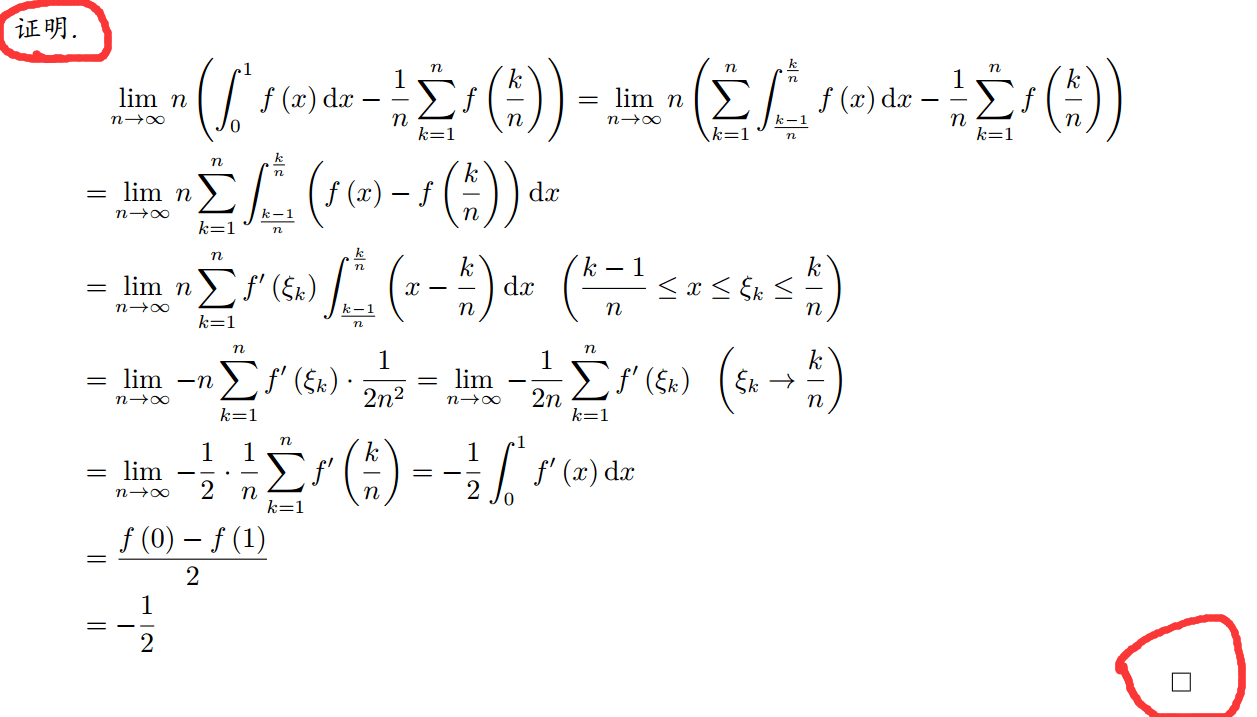
\includegraphics[width=.85\textwidth]{pic16}
\end{qst}
\ans 调用amsthm宏包。使用\mintinline{tex}{\newtheorem}自定义一个你要的不就行了?
 或者,你还可以使用 xsim 宏包,还可以控制分值,solution 的显示和隐藏。
 想用框还可以用tcolorbox宏包。
 
\begin{qst}\label{Q2018040407}
  一个1*3的矩阵 外围用了 pmatrix 括号有点问题。
\end{qst}
\ans 可以改变下思路。
 \begin{minted}{tex}
 \[
  \times
  \left(
  \left[\begin{aligned}1\\ i\\0\end{aligned}\right](M_0+M_2+M_4+M_6),
  \left[\begin{aligned}1\\-i\\0\end{aligned}\right](M_1+M_3+M_5+M_7),
  \left[\begin{aligned}0\\ 0\\1\end{aligned}\right](N_1+N_2+N_3+N_4)
  \right)
  \times {\mathrm e}^{i\frac{u\cos\theta}{\sin^2\alpha}}\,{\mathrm d}\theta
 \]
 \end{minted}
 \[
 \times
 \left(
 \left[\begin{aligned}1\\ i\\0\end{aligned}\right](M_0+M_2+M_4+M_6),
 \left[\begin{aligned}1\\-i\\0\end{aligned}\right](M_1+M_3+M_5+M_7),
 \left[\begin{aligned}0\\ 0\\1\end{aligned}\right](N_1+N_2+N_3+N_4)
 \right)
 \times {\mathrm e}^{i\frac{u\cos\theta}{\sin^2\alpha}}\,{\mathrm d}\theta
 \]
 
\begin{qst}\label{Q2018040408}
  不知道他们说的Better Bibtex是什么?\index{Better Bibtex}
\end{qst}
\ans Better BibTeX 是 Zotero 的一个插件,可以让Zotero 导出 .bib 档时设置一些选项。

\begin{qst}\label{Q2018040409}
  biblatex可以继续用bib文件来生成参考文献吗?
\end{qst}
\ans bibtex 要转用 biblatex 只需这么做:
 \begin{minted}{tex}
 \usepackage[backend=biber,style=ieee]{biblatex}  % style 在这里!
 \addbibresource{yourfile.bib}
 \end{minted}
然后主文不要用\mintinline{tex}{\bibliographystyle \bibliography},
直接\mintinline{tex}{\printbibliography}就行。

\begin{qst}\label{Q2018040410}
  biblatex有没有对应于abbrvnat那样的style?
\end{qst}
\ans 试试\mintinline{tex}{\usepackage[style=trad-abbrv,natbib,backend=biber]{biblatex}}。
还可以看看biblatex-trad宏包。
\begin{center}
	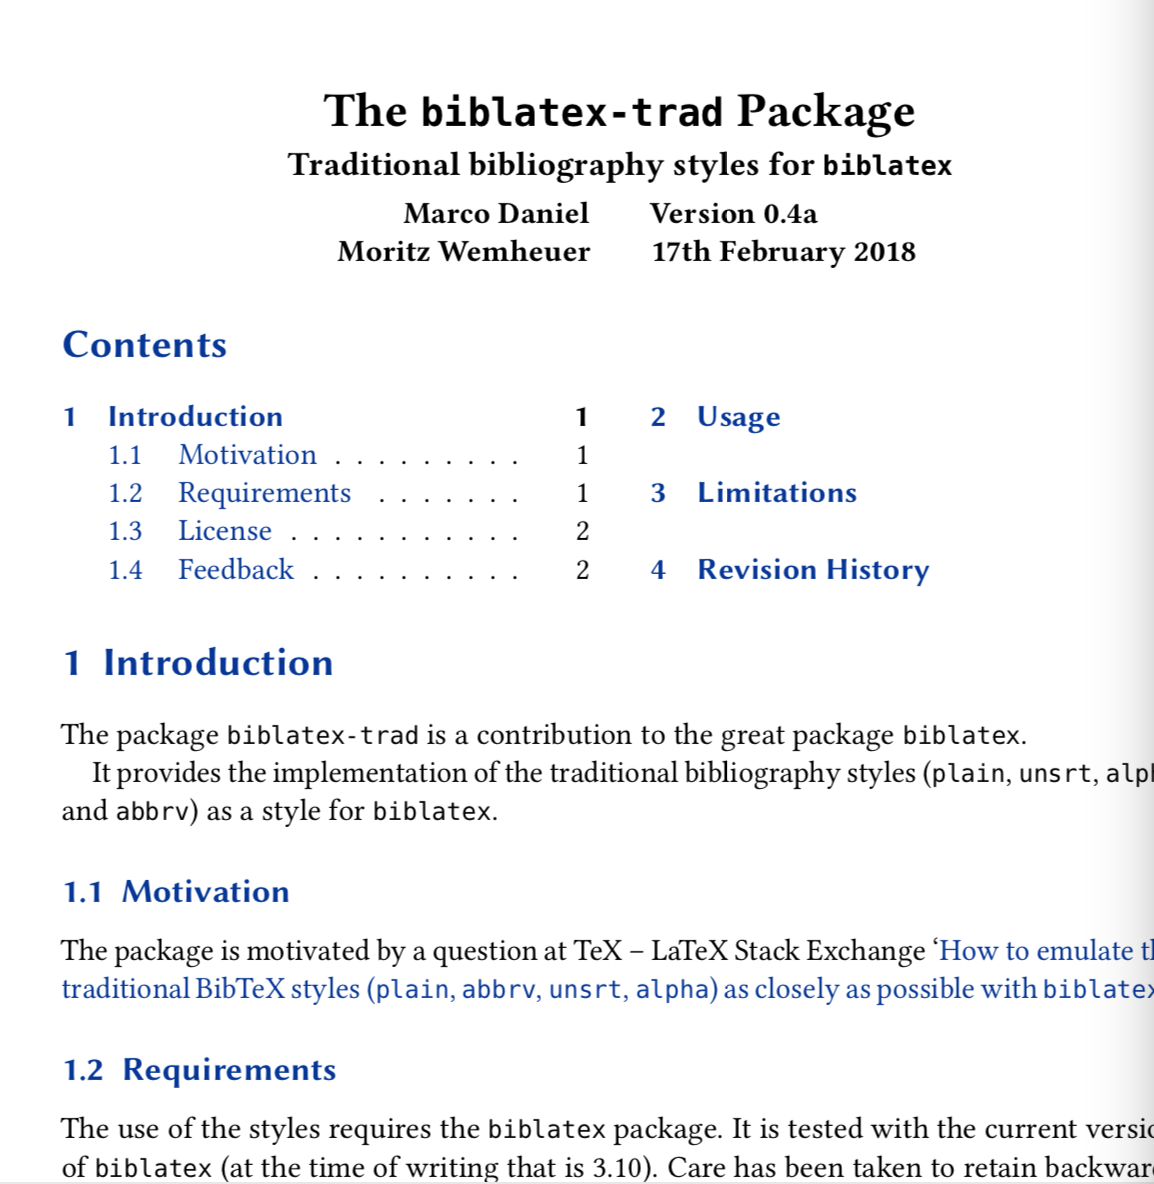
\includegraphics[width=.65\textwidth]{pic17}
\end{center}

\begin{qst}\label{Q2018040411}
  中文加粗有什么方法?
\end{qst}
\ans 加粗多是英文的概念,中文的加粗,则是通过更改字体更合理,因为中文的笔划较多。
比如宋体,加粗可以设置粗宋、小标宋、宋黑。
再比如,黑体、大黑、中粗黑。
你得知道使用的正文字体文件是否有 bold 版本。
一般 windows 下为你配置的中易宋体是没有粗体字重的,
 \mintinline{tex}{\bfseries} 或 \mintinline{tex}{\textbf{文字}} 只是为你切换到中易黑体。
 
\begin{qst}\label{Q2018040412}
  数学公式中如何实现任意内容堆叠?
\end{qst}
\ans 可以定义mathop。
 \begin{minted}{tex}
\[
 \mathop{L(x,y)}\limits_{\rho(x,y)\to 0}\to A\bigl(1-{\mathrm e}^{-kd(x,y)}\bigr)
\]
 \end{minted}
 \[
   \mathop{L(x,y)}\limits_{\rho(x,y)\to 0}\to A\bigl(1-{\mathrm e}^{-kd(x,y)}\bigr)
 \]
\end{document} 